%%%%%%%%%%%%%%%%%%%%%%%%%%%%%%%%%%%%%%%%%%%%%%%%%%%%%%%%%%%%%%%%%%%%%%%%%%%%%%%
%%   Created by                                                              %%
%%   Dr Varun Ojha, extended by Julian K, Christopher Maynard                %%
%%   Lecturer, Department of Computer Science                                %%
%%   University of Reading, UK                                               %%
%%                                                                           %%
%%%%%%%%%%%%%%%%%%%%%%%%%%%%%%%%%%%%%%%%%%%%%%%%%%%%%%%%%%%%%%%%%%%%%%%%%%%%%%%
%%%%     SETTING STARTS - DO NOT CHANGE Unless your Tex setting require so   %%
%%%%%%%%%%%%%%%%%%%%%%%%%%%%%%%%%%%%%%%%%%%%%%%%%%%%%%%%%%%%%%%%%%%%%%%%%%%%%%%
%%----------------------------------------------------------------------------------
% DO NOT Change this is the required setting A4 page, 11pt, onside print, book style
%%----------------------------------------------------------------------------------
\documentclass[a4paper,11pt]{article}

%%-------------------------------------
%% Page margin settings - % half inch margin all sides (recommended)
%%-------------------------------------
\usepackage[margin=1.2in]{geometry}

%%-------------------------------------
%% Font settings - % CM San or Arial (recommended)
%%-------------------------------------
% Switch the following two line off: to revert back to defult LaTex font (NOT recomended)
\usepackage{amsfonts}
\renewcommand*\familydefault{\sfdefault}

%%-------------------------------------
%% Math/Defination/Theorem/Algorithm packages settings
%%-------------------------------------
\usepackage[cmex10]{amsmath}
\usepackage{amssymb}
\usepackage{amsthm}
\newtheorem{mydef}{Definition}
\newtheorem{mytherm}{Theorem}

% Header footer
\usepackage{fancyhdr}

%%-------------------------------------
%% Algorithms/Code Listing environment settings  -
%% Please do not change these settings
%%-------------------------------------
\usepackage{algorithm}
\usepackage{algpseudocode}
\renewcommand{\algorithmicrequire}{\textbf{Input:}}
\renewcommand{\algorithmicensure}{\textbf{Output:}}
\usepackage[utf8]{inputenc}
\usepackage{listings}
\usepackage{xcolor}
\definecolor{codegreen}{rgb}{0,0.6,0.1}
\definecolor{codegray}{rgb}{0.5,0.5,0.5}
\definecolor{codeblue}{rgb}{0.10,0.00,1.00}
\definecolor{codepurple}{rgb}{0.58,0,0.82}
\definecolor{backcolour}{rgb}{1.0,1.0,1.0}
\lstdefinestyle{mystyle}{
    backgroundcolor=\color{backcolour},
    commentstyle=\color{codegreen},
    keywordstyle=\color{codeblue},
    numberstyle=\tiny\color{codegray},
    stringstyle=\color{codepurple},
    basicstyle=\ttfamily\footnotesize,
    breakatwhitespace=false,
    breaklines=true,
    captionpos=b,
    keepspaces=true,
    numbers=left,
    numbersep=5pt,
    showspaces=false,
    showstringspaces=false,
    showtabs=false,
    tabsize=2,
    frame=none
}
\lstset{style=mystyle}

%%-------------------------------------
%% Graphics/Figures environment settings
%%-------------------------------------
\usepackage{graphicx}
\graphicspath{{./figures/}}
\usepackage{subfigure}
\usepackage{caption}
\usepackage{titling}

%%-------------------------------------
%% Table environment settings
%%-------------------------------------
\usepackage{multirow}
\usepackage{rotating}
\usepackage{makecell}
\usepackage{booktabs}
%\usepackage{longtable,booktabs}

%%-------------------------------------
%% List of Abbreviations settings
%%-------------------------------------
\usepackage{enumitem}
\newlist{abbrv}{itemize}{1}
\setlist[abbrv,1]{label=,labelwidth=1in,align=parleft,itemsep=0.1\baselineskip,leftmargin=!}

%%-------------------------------------
%% bibliography/Refernces settings   - Harvard Style was used in this report
%%-------------------------------------
\usepackage[hidelinks]{hyperref}
\usepackage{cleveref}
\usepackage[comma,authoryear]{natbib}
\renewcommand{\bibname}{References} % DO NOT remove or switch of

%% Code style
\definecolor{pblue}{rgb}{0.13,0.13,1}
\definecolor{pgreen}{rgb}{0,0.5,0}
\definecolor{pred}{rgb}{0.9,0,0}
\definecolor{pgrey}{rgb}{0.46,0.45,0.48}
\lstset{
	basicstyle=\ttfamily\footnotesize,
	numberstyle=\ttfamily\tiny,
	frame=single,
	numbers=left,
	numbersep=1em,
	xleftmargin=2em,
	language=C++,
	breaklines=true,
	breakatwhitespace=true,
	postbreak=\hbox{$\hookrightarrow$ },
	showstringspaces=false,
	tabsize=2,
	commentstyle=\color{pgreen},
	keywordstyle=\color{pblue},
	stringstyle=\color{pred},
	moredelim=[il][\textcolor{pgrey}]{\[\]},
	moredelim=[is][\textcolor{pgrey}]{\%\%}{\%\%},
  columns=fullflexible,
	upquote=true
}
\usepackage{attachfile}
\usepackage{float}
\usepackage{pdfpages}

\floatstyle{plain}

\newfloat{lstfloat}{htbp}{lop}
\floatname{lstfloat}{Listing}
\def\lstfloatautorefname{Listing} % needed for hyperref/auroref

%%-------------------------------------
%% Appendix settings
%%-------------------------------------
\usepackage[toc]{appendix}

%% HDR Footer
\fancypagestyle{plain}{%
  \fancyhf{}
  \fancyhead[R]{\slshape \rightmark}
  \fancyhead[L]{\slshape \leftmark}
  \fancyfoot[C]{CS1PR16 Programming Project}
  \fancyfoot[L]{\theauthor}
  \fancyfoot[R]{\thepage} % /\pageref*{pg:lastpage}
  \renewcommand{\headrulewidth}{0.4pt}
  \renewcommand{\footrulewidth}{0.4pt}
}
\pagestyle{plain}

%%%%%%%%%%%%%%%%%%%%%%%%%%%%
%%%%%  USER SETTINGS   %%%%%
%%%%%%%%%%%%%%%%%%%%%%%%%%%%
\title{Extending a platform game in C/C++: You can give your extensions a nice title}
\author{Firstname Lastname}

%%%%%%%%%%%%%%%%%%%%%%%%%%%%%
%%%%%   SETTING ENDS   %%%%%%
%%%%%%%%%%%%%%%%%%%%%%%%%%%%%
\begin{document}
    \captionsetup[figure]{margin=1.5cm,font=small,name={Figure},labelsep=colon}
    \captionsetup[table]{margin=1.5cm,font=small,name={Table},labelsep=colon}

    %\frontmatter

    \begin{titlepage}
        \begin{center}
            
\includegraphics[width=3cm]{figures/uorlogo.png}\\[0.5cm]
            {\LARGE University of Reading\\[0.5cm]
                Department of Computer Science}\\[2cm]
            %{\color{blue} \rule{\textwidth}{1pt}}

            %------------------------------  TITLE of Your PROJECT ----------------------------------%
            % change the following line
            \linespread{1.2}\huge {\thetitle}


            \linespread{1}~\\[2cm]
            %{\color{blue} \rule{\textwidth}{1pt}}

            %------------------------------  Your Name  -------------------------------%
            {\Large \theauthor} \\[1cm]



            % Input here the correct information:
            \normalsize
            \vfill
            \begin{tabular}{lp{10cm}}
            Module Code & CS1PR16 \\
            Assignment report Title &  Programming Project \\
            Student Number (e.g. 25098635)        & TODO \\
            Date (when the work completed)        & \today \\
            Actual hrs spent for the assignment   & TODO   \\
            Assignment evaluation (3 key points)  & TODO Enter here your comments: engaging task, learned something, could improve the description about XXX
            \end{tabular}
        \end{center}
    \end{titlepage}

    % -------------------------------------------------------------------
    % Declaration
    % -------------------------------------------------------------------
    \newpage
    %\mainmatter
    \section*{\Large Declaration}
    % PLEASE CHANGE THIS TEXT EXCEPT YOUR NAME%
    % -------------------------------
    % PLEASE ONLY UPDATE HERE -- PLEASE WRITE YOUR NAME %
    % -------------------------------
    I, \textbf{\theauthor}, of the Department of Computer Science, University of Reading, confirm that all the sentences, figures, tables, equations, code snippets, artworks, and illustrations in this report are original and have not been taken from any other person's work, except where the works of others have been explicitly acknowledged, quoted, and referenced. I understand that if failing to do so will be considered a case of plagiarism.
    Plagiarism is a form of academic misconduct and will be penalised accordingly.\\[1cm]


    \begin{flushright}
        \textbf{\theauthor}

        \today
    \end{flushright}
    \let\cleardoublepage\relax

    \tableofcontents
    %\listoffigures
    %\listoftables

    % -------------------------------------------------------------------
    % Main chapters and sections of your Project
    % Everything from here on your words and works
    % -------------------------------------------------------------------
    \newpage
    % Read for preparation of document in LaTex
    % Lamport, L. (1986), LATEX: A Document Preparation System, Addison-Wesley.

    \section{Introduction}

%This template was produced using the \LaTeX type-setting system. It is
%more powerful than a WISIWIG word processor system such as Microsoft
%Word, especially when it comes to type-setting for code listings.
%See the text in the {\texttt{*.tex}} files for how to do this. A text editor such as
%Atom is suitable for writing the {\texttt{*.tex}} file. For more
%information on using \LaTeX~see~\cite{latex1} - an electronic resource
%from the library or see~\cite{latex2} for an online guide. You are
%free to use a word processor if you wish. Use this guide as a template
%for your report.
The aim of the project is to assess your ability to analyze, design
and implement an extension to an existing C/C++ program. The given program is a platform game that uses the SLD2 library for the graphics.

Your task is to extend the platform game starting from the provided skeleton code.
Hence, you must design at least one new feature, then adapt, modify and develop the code to realize this feature.
You are free to add any features you wish. You are required to write a
report describing the design and implementation of the changes you
make. You may develop it under Windows or Linux on the machines in the CS labs or on your own machine.

The assessment will take the form of a report on the game you develop.
You will be assessed on the complexity of your contribution and the quality of the report to document this contribution.The code will not be directly assessed although you must include a diff from your gitlab repository from the initial repository to the finished version.

\subsection{Learning Objectives}
\begin{itemize}
  \item Designing and implementing larger program in C/C++
  \item Managing the project development
  \item Report writing
\end{itemize}

\subsection{Provided Code}

You have been provided with a skeleton of a platform game which you
imported into the Visual Studio IDE in the tutorial for Week 1.
This skeleton uses the SLD2 library for graphics, sound, and keyboard interaction.
In Week 5, the tutorial was to follow the online tutorial from {\texttt{parallelrealities.co.uk}} on how the program had been constructed.

The skeleton code is written in C using {\em structs} as the main
data structure. You are free to develop the code in this style or to enrich it using C++ classes using an object orientation style.
Either way, you must justify you choice in the report and demonstrate this was
a sensible choice for the features you have employed.

\subsection{Suggested Approach}

You should use the practical session in G56 on Mondays, the drop-in
session on Mondays (G45), the CS1PR Slack channel and the programming
angel scheme to access help and support.
You may also help and receive
help from fellow students.
However, you should bare in mind this is an individual project make sure you submit only your own work.
See the University guidelines on plagiarism which are online.  

Your report should start with an {\textbf{Introduction}} section where
you introduce your work. What were the project goals, what features
did you wish to include in the game. Think about features of platform games you have played that
improve the game play. You may wish to include some of the following,
high scores, multiple levels, power-ups, enemies, movement parts
{\em etc}. 
You should justify what
programming style such as C/C++, did you use any OO features {\em etc}.

\section{Design}
Document what features you decided to implement and how they interact with
the rest of the game. Explain how the game play works.  
Include a diagram such as a flow
chart, \Cref{fig:fc} or UML diagram, \Cref{fig:uml}\footnote{Including
  both is allowed or even encouraged.}.

\begin{figure}[H]
\centering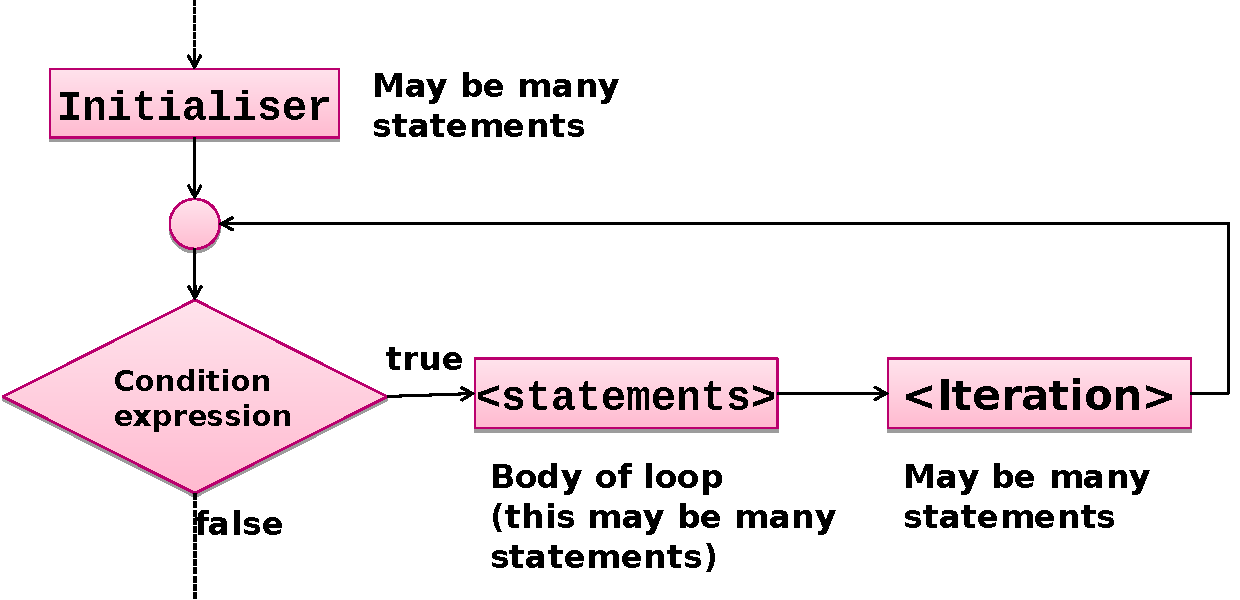
\includegraphics[width=0.66\linewidth]{simple-fc.pdf}
\caption{\label{fig:fc}A simple figure}
\end{figure}

\begin{figure}[H]
\centering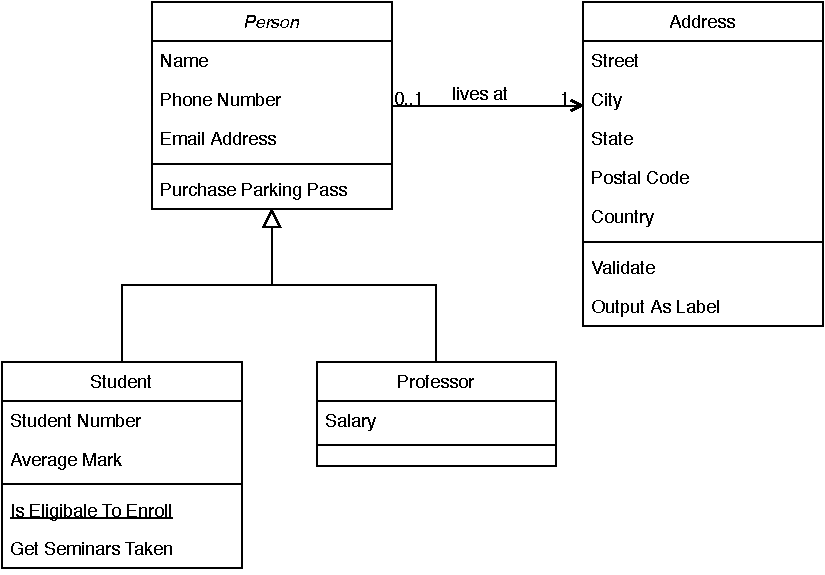
\includegraphics[width=0.75\linewidth]{simple-uml.pdf}
\caption{\label{fig:uml}A simple UML class diagram}
\end{figure}

In \Cref{lst:example}, you can see how to present a code example.
You can refer to specific sections of code using the line numbers, e.g., between Line~5-10, the setup is made, ...

\begin{lstfloat}
\lstinputlisting[label=lst:example,caption=My testcode (example.cpp) \attachfile{code/example.cpp}]{code/example.cpp}
\end{lstfloat}

\section{Implementation and Development}
Describe how you developed the code including what language features
you employed and why.
How did your program evolve from the original design?
Did you adapt the design to improve the game?
You should include code fragments and screen shots illustrate particular features.

Describe the finished game, including all the features you added.
What features work well?
Document any parts of the code which feel are important or
enable the program to work in a particular way.

Describe here your journey how you developed the program and reflect about your development.
How did you test and debug the program? Did you find all the bugs?
What testing have you employed to ensure the game works correctly. Did
you use any specific strategies for testing? 


\section{Conclusion}
Summarise your program development. What have your learnt about
programming? What have you learnt about developing a significant
program. What would either features would you add if you had more
time. What would you do differently?

    % -------------------------------------------------------------------
    % References  -  Harvard Style was used in this report
    % -------------------------------------------------------------------
    \bibliographystyle{agsm} % Harvard Style

    \nocite*
    \bibliography{references}  %  Patashnik, O. (1988), BibTEXing. Documentation for general BibTEX users.
    \label{pg:lastpage}

    \newpage
    \begin{appendices}
      \section{Code Changes}
Repository: \url{https://csgitlab.reading.ac.uk/di918039/cs1pr-portfolio}.

Reference the URL of your code repository (that you made accessible to us).
Include a {\texttt diff} of your code repository on CSGitlab from the provided skeleton code; the intital {\texttt commit} (which is the code for Week 1 tutorial) and your final working version.

This can be achieved as follows:
In CSGitlab, go to your repository, select Repository, then Compare.
Now enter as Source "master" and as "target" the Git revision of the initial code and press "Compare".
You will see the history of commits and the detailed changes (deltas) to the original code.
Print this as PDF and include it here.

\textbf{To make this work: after you received the project code, commit the initial code without any changes.}

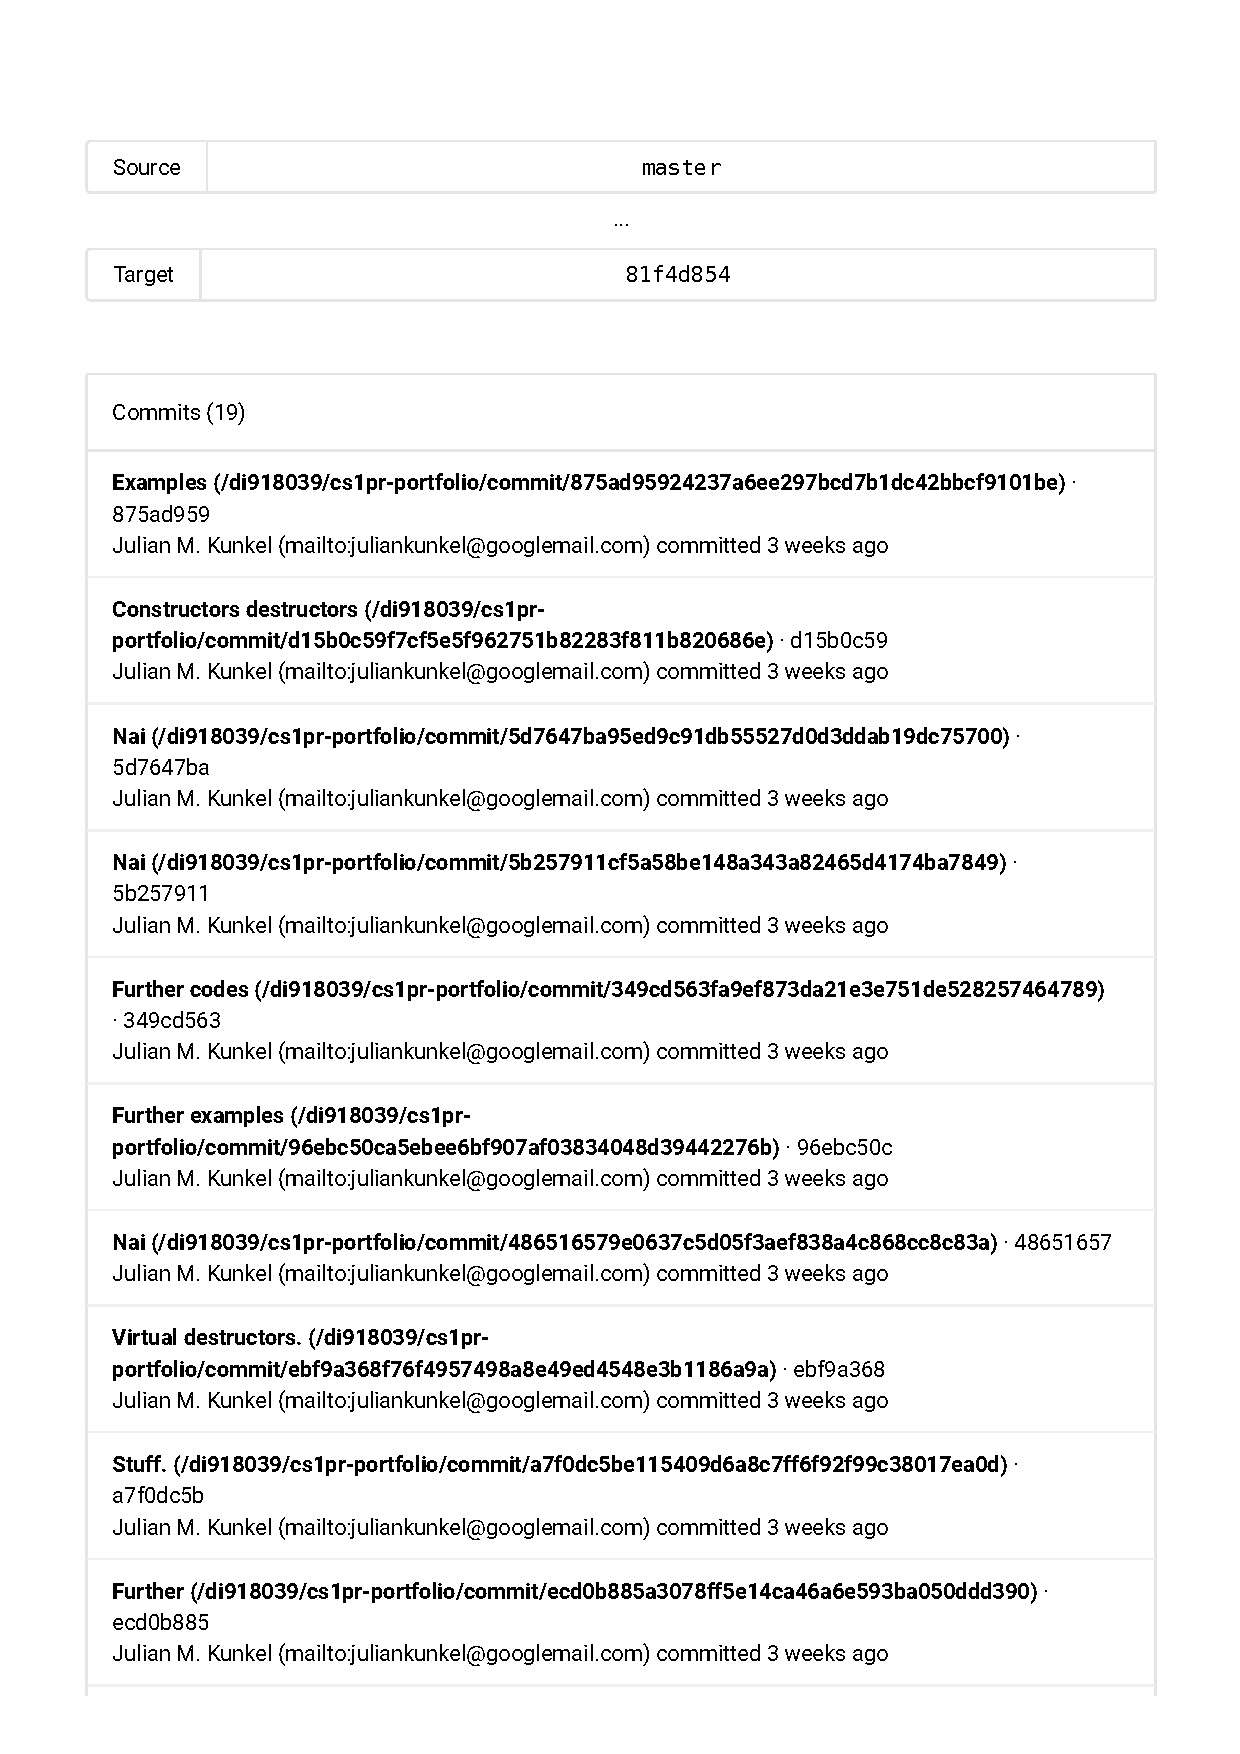
\includepdf[pages=-]{code-delta.pdf}

      % if you want to add further stuff
      % \input{appendix_extra.tex}
    \end{appendices}

\end{document}
